\documentclass{article}
\usepackage[utf8]{inputenc}
\usepackage[T1]{fontenc}
\usepackage{amsmath}
\usepackage{amsfonts}
\usepackage{amssymb}
\usepackage{enumitem}

\usepackage[margin=0.5in]{geometry} % Adjust the margins of document here.

\usepackage{tikz}                                          % Для простых рисунков в документе
\usetikzlibrary{matrix,arrows,decorations.pathmorphing,shapes.geometric,calc,snakes,backgrounds,arrows.meta}
\usepackage{xcolor}

\begin{document}

\section*{Problems (10 points max)}

\begin{enumerate}
  \item (2 points) Let $\xi$ and $\eta$ be independent random variables with exponential distributions, i.e., $$p_\xi(x) = p_\eta(x) = \lambda e^{-\lambda x} \theta(x)$$ where
  \[
  \theta(x) = 
  \begin{cases} 
  1, & \text{if } x \geq 0 \\
  0, & \text{if } x < 0 
  \end{cases}
  \]
  Find the following densities: $p_{\xi,\xi+\eta}(x, y)$ and $p_{\xi|\xi+\eta=z}(x)$. 
  
  \textbf{Important:} For the joint density, indicate the region where it equals zero.
  
  \item (2 points) Let $\xi$ and $\eta$ be two independent normal distributions with parameters $(a_1, \sigma^2_1)$ and $(a_2, \sigma^2_2)$. Find the density distribution of the vector $(\xi + \eta, \xi - \eta)$. Will the coordinates of this vector be independent?
  
  \item (2 points) Let $\xi$ and $\eta$ be independent random variables with distributions $\mathcal{N}(0,1)$. Find the density of the variable $\chi = \xi^2 + \eta^2$.
  
  \item (2 points) Random variables $X$ and $Y$ are independent. $X$ has a Laplace distribution 
  with density $\frac{1}{2}e^{-|x|}$, while $Y$ is uniformly distributed in the interval $[1, 2]$.
  \begin{enumerate}
    \item Find the distribution density of the random variable $-2Y$
    \item Find the distribution density of the random variable $X - 2Y$
  \end{enumerate}
  
  \item (2 points) Consider the following maze:

  \begin{center}    
    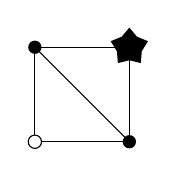
\begin{tikzpicture}[scale=0.6]
      % Drawing the square
      \draw (0,0) -- (0,2) -- (2,2) -- (2,0) -- cycle;
      
      % Drawing the diagonal
      \draw (0,2) -- (2,0);
      
      % Marking the vertices of the square
      \draw[fill=white] (0,0) circle (4pt);
      \fill (0,2) circle (4pt);
      \fill (2,0) circle (4pt);
      \node[star,fill=black,minimum width=1pt] at (2,2) {};
    \end{tikzpicture}
\end{center}

A person leaves the point marked with $\circ$, choosing a direction with 
equal probability and randomly and independently at each step. 
As a random variable $\xi$, consider the number of steps needed 
to first reach the point marked with star. 
Find the expected value of $\xi$.
\end{enumerate}
\end{document}
